\chapter{De la tipare secventiale frecvente la silabisire}
\label{cap:contributii}

În cadrul acestui capitol se prezenta în detaliu metoda propusă, prin care, pornind de tipare secvențiale frecvente, se pot identifica despărțiri în silabe ale cuvintelor.  

\section{Prezentare de ansamblu a soluției}

\begin{figure}[h]
    \centering
    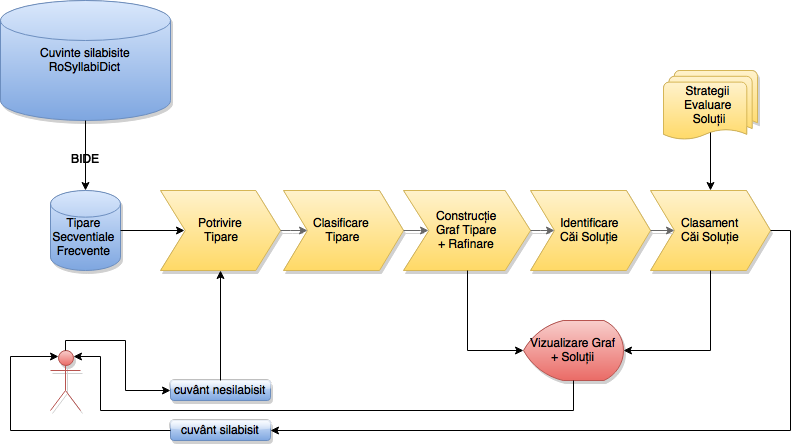
\includegraphics[width=\textwidth]{figures/rosil-flow.png}
    \caption{Diagrama conceptuală a soluției propuse}
    \label{fig:rosil-flow}
\end{figure}

Principalele etape ale metodei sunt următoarele:
\begin{enumerate}
\item Identificarea tiparelor frecvente dintr-un set de cuvinte despărțite în silabe și indexarea acestora.
\item Identificarea tiparelor care prezintă un grad ridicat de potrivire în cadrul cuvântului care se dorește a fi despărțit în silabe
\item Clasificarea acestor tipare în funcție poziția în cuvânt pe care au "potrivit-o" (început, sfârșit, interior).
\item Construirea unui graf cu aceste tipare pe baza potrivirii dintre aceste tipare
\item Eliminarea nodurilor izolate din acest graf
\item Pe baza unor strategii de predicție, se va alege o cale sau mai multe în acest graf, reprezentând soluția propusă sau soluțiile soluțiile propuse pentru despărțirea în silabe.
\end{enumerate}

\section{Identificarea tiparelor frecvente}

Pentru a construi setul de tipare frecvente a fost folosită colecția de cuvinte despărțite în silabe în limba română RoSyllabiDict, \cite{bib:BARBU08.495}. Acest set de date conține 525486 de cuvinte despărțite în silabe. 

În vederea analizei setului de date, în cadrul tabelului \ref{table:sdb_counts} se poate observa variația numărului de tipare secvențiale frecvente închise în funcție de valoarea suportului minim.   

\begin{table}[h!]
\centering
\begin{tabular}{|c|c|c|c|c|c|c|c|c|}
\hline
Sup.& Total & Lung. 1 & Lung. 2 & Lung. 3 & Lung. 4 & Lung. 5 & Lung. 6 & Lung. 7\\ 
\hline
\hline
1000 & 648 & 252 & 385 & 11 & 0 & 0 & 0 & 0\\ 
\hline
800 & 890 & 293 & 576 & 21 & 0 & 0 & 0 & 0\\ 
\hline
600 & 1339 & 380 & 903 & 56 & 0 & 0 & 0 & 0\\ 
\hline
400 & 2211 & 523 & 1544 & 143 & 1 & 0 & 0 & 0\\ 
\hline
200 & 4812 & 832 & 3384 & 576 & 20 & 0 & 0 & 0\\ 
\hline
100 & 10461 & 1234 & 6754 & 2309 & 162 & 2 & 0 & 0\\ 
\hline
50 & 22852 & 1824 & 12671 & 7453 & 853 & 47 & 4 & 0\\ 
\hline
20 & 62549 & 2597 & 25731 & 28056 & 5384 & 674 & 90 & 17\\ 
\hline
10 & 129106 & 3271 & 41126 & 63388 & 17812 & 2940 & 454 & 97\\ 
\hline
5 & 256065 & 4146 & 63443 & 123429 & 52271 & 10553 & 1840 & 327\\ 
\hline
2 & 633195 & 5469 & 104254 & 248227 & 186623 & 66915 & 16920 & 3882\\ 
\hline\end{tabular}
\label{table:sdb_counts}
\caption{Numărul de tipare frecvente închise pentru setul de date RoSyllabiDict} 
\end{table}

Alegerea unui suport minim cat mai mic asigură prezența a cât mai multor tipare în colecția de tipare folosite ulterior de metodă. Aceasta va creste precizia metodei, dar pe de altă parte va avea o influentă negativă asupra timpului de execuție. 

Cu cât numărul de tipare este mai mare, cautarea de potriviri devine mai lentă, iar pentru a creste performanța, acestea pot fi indexate. În tabelul \ref{table:sdb_patterns} sunt prezentate o serie de tipare frecvente. Pentru a le indexa metoda se folosește de o tabela de disperie în care valorile cheilor vor fi reprezentate de silabele concatenate continute de tipare. Un astfel de exemplu se regăseste în cadrul tabelului \ref{table:sdb_index}. 

\begin{table}[h!]
\centering    
\begin{tabular}{|l|l|}    
\hline      
Cheie & Valoare\\
\hline
$a$ 		& $(<a>, 2)$  \\
$libe$ 		& $(<li, be>, 2)$  \\
$programa$ 	& $(<pro, gra, ma>, 2)$  \\
$mare$ 		& $(<ma, re>, 2)$  \\
$mator$ 	& $(<ma, tor>, 2)$  \\
$ti$ 		& $(<ti>, 2)$  \\
$eli$ 		& $(<e, li>, 3)$  \\
$grama$ 	& $(<gra, ma>, 3)$  \\
$sare$ 		& $(<sa, re>, 3)$  \\
$tor$ 		& $(<tor>, 4)$  \\
$li$ 		& $(<li>, 4)$  \\
$e$ 		& $(<e>, 5)$  \\
$ma$ 		& $(<ma>, 5)$  \\
$re$ 		& $(<re>, 6)$  \\
\hline
\end{tabular}
\caption{Exemplu de indexare pentru tipare secvențiale frecvente}
\label{table:sdb_index}               
\end{table}  

Odată având colecția de tipare frecvente indexată, procesul de silabizarea poate fi initial. 
 
\section{Potrivirea tiparelor in vederea silabisirii}

Fie $w$ un cuvânt compus dintr-o secvență de litere, iar $Z_w$ mulțimea tuturor subsecventelor continue ale acestui cuvânt, precum si îndexii de inceput și sfârșit ai acestora.

\begin{ex}
Pentru cuvântul $amator$, tuplele din multimea sunt $Z_{amator}$ sunt ilustrate în cadrul tabelului \ref{table:sdb_substrings}. 
\end{ex}


\begin{table}[h!]
\centering    
\begin{tabular}{|l|l|}    
\hline      
Secventă & Indexi\\
\hline
$a$ 		& $\left[0,1\right), \left[2,3\right)$  \\
$m$ 		& $\left[1,2\right)$  \\
... 		& ...  \\
$amator$ 	& $\left[0,6\right)$  \\

\hline
\end{tabular}
\caption{Mulțimea $Z_{amator}$}
\label{table:sdb_substrings}               
\end{table}  

\begin{defi} Prin \textbf{potrivirea tiparelor} pentru cuvântul $w$, având multimea $Z_w$ asociată, se dorește identificarea tuturor tiparelor frecvente care sunt indexate cu chei care aparțin multimii $Z_w$. Notăm rezultatul acestei operații cu $M_w$. Considerând același cuvânt $amator$, $M_{amator}$ este ilustrată în tabelul \ref{table:sdb_pattern_match}
\end{defi}

\begin{table}[h!]
\centering    
\begin{tabular}{|l|l|}    
\hline      
Tipar frecvent & Indexi potrivire\\
\hline
$(<a>, 2)$			& $\left[0,1\right), \left[2,3\right)$   \\
$(<ma>, 5)$  		& $\left[2,4\right)$\\
$(<ma, tor>, 2)$ 	& $\left[2,6\right)$ \\
$(<tor>, 4)$  		& $\left[4,6\right)$\\
\hline
\end{tabular}
\caption{Exemplu de potrivire de tipare pentru $Z_{amator}$}
\label{table:sdb_pattern_match}               
\end{table}  

Pentru ca ulterior sa se poată identifica posibile despărțiri în silabe este necesară clasificarea tiparelor frecvente potrivite. Astfel, există patru tipuri de tipare:  

\begin{itemize}
\item tipare de \textbf{început}: ($<a>$,2),
\item tipare \textbf{intermediare}: ($<ma>$,5), ($<a>$,2).
\item tipare de \textbf{sfârșit}: ($<ma, tor>$,2), ($<tor>$,4).  
\item tipare \textbf{complete} (acele tipare frecvente care inglobeaza întreg cuvântul de despărțit).
\end{itemize}

Odată identificate aceste tipare frecvente se pune problema organizării acestora în vederea reconstrucției cuvântului din tipare frecvente. Aceste reconstrucții pot reprezinta posibile despătiri corecte în silabe. 

Pentru această reconstrucție s-a ales ca structură de date un graf orientat, după cum va fi descris în secțiunea următoare.

\section{Grafuri de tipare}

În cazul tiparelor frecvente, trebuie remarcat faptul că, în majoritatea cazurilor, există legături între acestea. Prin legături între tipare se înțelege ca fie unele se termină în vecinătatea unei litere dintr-un cuvânt, iar altele încep în acea poziție, sau chiar mai mult decat atat, există tipare între care există suprapuneri. 

Pornind de la aceste obervații, în cele ce urmează, va fi arătat că pe baza acestor relatii dintre tiparele frecvente ale unui cuvânt, se vor putea construi \textbf{lanțuri de tipare secvențiale frecvente}, care să reprezinte silibisiri ale cuvântului respectiv.

\subsection{Construcția grafului de tipare secvențiale frecvente}
\begin{defi}
Fie $p_1$ și $p_2$ doua tipare de forma  $\langle s_1,sup_{s_1}, \left[i_{s_1},j_{s_1}\right) \rangle$, $\langle s_2,sup_{s_2}, \left[i_{s_2},j_{s_2}\right)\rangle $, potrivite în cadrul cuvântului $w$. $p_1 \curvearrowright p_2$ ($p_1$ este extins de $p_2$) dacă $i_{s_1} \epsilon \left[0, i_{s_2}\right)$ și $j_{s_1}\in $ \textit{mulțimii indexilor de despărțire ai tiparului} $s_2$. 
\end{defi}

\begin{ex}
Pentru cuvântul \textit{amator}, cu multimea tiparelor potrivite $M_{amator}$ descrisă în tabelul \ref{table:sdb_pattern_match} există o serie de extinderi de tipare descrise în cadrul tabelului \ref{table:sdb_pattern_extensions}
\end{ex}

\begin{table}[h!]
\centering    
\begin{tabular}{|l|l|}    
\hline      
$p_1$ & $p_2$\\
\hline
$\langle<a>, 2, \left[0,1\right)\rangle$ & $\langle<ma>, 5, \left[1,3\right)\rangle$  \\
$\langle<a>, 2, \left[0,1\right)\rangle$ & $\langle<ma,tor>, 2, \left[1,6\right)\rangle$  \\
$\langle<ma>, 5, \left[1,3\right)\rangle$ & $\langle<tor>, 4, \left[3,6\right)\rangle$  \\
$\langle<a>, 2, \left[2,3\right)\rangle$ & $\langle<tor>, 4, \left[3,6\right)\rangle$  \\
\hline
\end{tabular}
\caption{Extiderile $p_1 \curvearrowright p_2$ pentru $M_{amator}$}
\label{table:sdb_pattern_extensions}               
\end{table}  

\begin{defi}
Fie $P_w$ o multime de tipare secvențiale frecvente ale cuvântului $w$ și mulțimea perechilor de extensii pentru tiparele secventiale frecvente: 
\begin{equation}
E_w = \{\langle p_i, p_j \rangle \vert p_i,p_j \in P_w \wedge p_i \curvearrowright p_j\}
\end{equation}
Un \textbf{graf de tipare frecvente} pentru cuvântul $w$, este $G_w = \langle P_w, E_w \rangle$, unde $P_w$ este mulținea nodurilor, iar $E_w$ mulțimea muchiilor. 
\end{defi}

\begin{ex}
În cadrul figurii \ref{fig:rosil-amator} este prezentat graful $G_{amator}$. Nodul gri reprezintă un nod de start, nodurile albastre sunt noduri intermediare, iar nodurile roșii reprezintă noduri terminale. 
\end{ex}

\begin{figure}[h!]
    \centering
    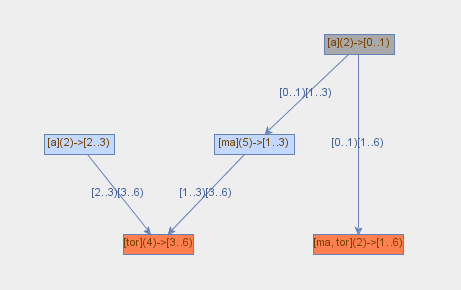
\includegraphics[width=0.7\textwidth]{figures/rosil-amator.png}
    \caption{Graful de tipare pentru cuvântul \textit{amator}}
    \label{fig:rosil-amator}
\end{figure}

\subsection{Interpretarea grafului de tipare frecvente}

Odată construit graful de tipare frecvente, se pune întrebarea dacă pe baza acestuia, se poate dezvolta o metodă de silabisire? 

În graful prezentat în figura \ref{fig:rosil-amator} se pot observa trei dintre cele patru tipuri de tipare (de început, de sfârsit, întermediare), stiind aceasta, se ridică întrebarea dacă caile dintre noduri de început și sfârșit reprezintă posibile despărțiri în silabe, iar dacă, care dintre acestea este despărțirea corectă?

În cazul exemplu prezentat există doua căi între noduri de început si sfârsit, acestea fiind $<a>, <ma, tor>$, respectiv $<a>, <ma>, <tor>$. Din ambele variante se ajunge la despărțirea în silabe $a-ma-tor$, care este si varianta corectă. 

Pornind de la această observație, în cele ce urmează vor fi prezentate o serie de strategii de selecție a căilor dintr-un graf de tipare frecvente care au probabilitate ridicată sa fie despărțiri în silabe corecte. 

Dar până se ajungă la aceste strategii trebuie menționat că în realitate, numărul de tipare frecvente potrivite cu un cuvânt este mult mai mare decât în exemplu demonstrativ din figura \ref{fig:rosil-amator}, iar cum căutarea tuturor căilor între două noduri este o problemă dificilă, a carei soluție depinde de complexitatea grafului analizat, este recomandată o reducere a dimensiunii grafului pentru a reduce complexitatea cautării. 

\subsection{Optimizarea grafului de tipare frecvente}

Pornind de la observația de mai sus și analizând natura grafurile de tipare, se pot identifica două categorii de noduri a căror utilitate este inexistentă în vederea identificării căilor între noduri de început și noduri de sfârsit. Aceste categorii sunt:
\begin{itemize}
\item nodurile la care nu se poate ajunge din niciun nod de start.
\item nodurile din care nu se poate ajunge la niciun nod de sfârșit. 
\end{itemize}


\begin{ex}
În cadrul figurii \ref{fig:rosil-amator-prunned} se poate observa graful de tipare $G_{amator}$ după eliminarea nodurilor izolate.
\end{ex}

\begin{figure}[h!]
    \centering
    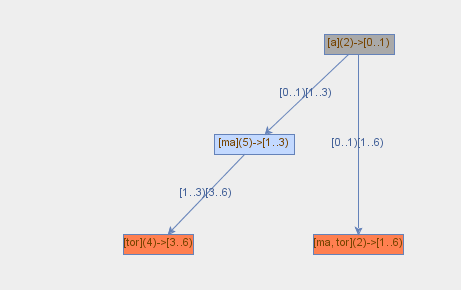
\includegraphics[width=0.6\textwidth]{figures/rosil-amator-prunned.png}
    \caption{Graful de tipare pentru cuvântul \textit{amator}}
    \label{fig:rosil-amator-prunned}
\end{figure}

Aceste noduri pot fi eliminate fără a altera soluțiile de silabisire identificate. O posibilă soluție pentru eliminarea acestora este descrisă în cadrul algoritmului \ref{algo:prunning}. 

Acesta are două etape: 
\begin{itemize}
\item O primă etapă în cadrul căreia sunt identificate nodurile care nu sunt noduri de sfârșit și nu există nicio muchie care să pornească de la acestea, respectiv nodurile care nu sunt noduri de început și pentru care nu există nicio muchie care să ajungă la ele.
\item Odată identificate aceste noduri, trebuie identificate și muchile care le au ca sursă sau destinație.
\end{itemize}

Eliminând nodurile izolate după aceste două etape, rezultă un graf de dimensiune mai mică. Cele două etape se aplică recursiv până când în cadrul primei etape nu mai este identificat niciun nod izolat. 

\begin{algorithm}[h!]
\SetAlgoLined
\SetKwFunction{ppg}{prunePatternGraph}

\ppg($G_{w}$) \\
\KwData{$G_{w}$ un graf de tipare descris prin $\langle V_w, E_w \rangle$}
\KwResult{$G_w'$ un graf fără noduri izolate} 

$isolatedVertices = \emptyset$ \\
\For{ $v$ \textbf{in} $V_w$}{
	\If{$deg^-(v) == 0 \wedge isNotStartNode(v)$} {
		$isolatedVertices = isolatedVertices \cup \{v\}$
	}
	\If{$deg^+(v) == 0 \wedge isNotEndNode(v)$} {
		$isolatedVertices = isolatedVertices \cup \{v\}$
	}
}

\If{$isolatedVertices == \emptyset$} {
	\KwRet $\langle V_w, E_w \rangle$
}


$edgesToBeRemoved = \emptyset$ \\
\For{ $e$ \textbf{in} $E_w$}{
	\If{$e$ \textbf{depends on a vertex from} $isolatedVertices$} {
		$edgesToBeRemoved = edgesToBeRemoved \cup \{e\}$
	}
}

$V_w' = V_w \setminus isolatedVertices$\\
$E_w' = E_w \setminus edgesToBeRemoved$\\

\KwRet \ppg($\langle V_w', E_w'  \rangle$) \\
\vspace{.1cm}

\caption{Eliminarea nodurilor izolate din cadrul unui graf de tipare}
\label{algo:prunning}
\end{algorithm}

\section{Lanțuri închise de tipare secvențiale frecvente}

Pornind de la un graf de tipare, se pot elabora o serie de strategii prin care se stabilește care dintre căile de dintre nodurile de început și sfârșit reprezintă despărțirea corectă în silabe a cuvântului pe baza căruia a fost construit graful de tipare. 

Dar înainte de  a prezenta aceste strategii, este necesară o scurtă analiză a acestor căi.
\subsection{Identificarea căilor care pot reprezenta despărțiri în silabe}

Pentru a putea aplica strategiile menționate mai sus, este necesară identificarea tuturor căilor între nodurile de început și cele de sfârșit. Problema identificării tuturor câilor într-un graf este una dificilă dar în cazul grafurilor de tipare, datorită naturii lor, poate fi abordată (grafurile de tipare sunt grafuri orientate aciclice de dimensiune relativ redusă). 

\begin{defi}
Se notează cu $I_w$ intervalul minim care conține mulțimea tuturor indexilor care pot reprezenta puncte de despărțire pentru cuvântul $w$.
\end{defi}

\begin{defi}
Fie $p_1, p_2, ..., p_n$ o cale într-un graf de tipare $G_w$, cu $p_x$ un tipar potrivit de forma $\langle tipar_x, sup_x, \left[i_x,j_x\right)\rangle$, această cale este un \textbf{lanț de tipare închis} daca 
\begin{equation}
\bigcup_{1 \leq x \leq n} \left[i_x,j_x\right) = I_w
\end{equation}
Cu alte cuvinte, un lanț de tipare închis este o cale într-un graf de tipare, pentru care primul nod este \textit{un nod de început}, iar ultimul nod este \textit{un nod de sfârșit}.
\end{defi}

Cum ar putea fi identificată eficient multimea tuturor lanțurilor de tipare închise? Această întrebare rămâne descrisă. Pentru a valida metoda descrisă în cadrul acestui experiment una dintre variante este ca din fiecare nod start să se realizeze explorări în lătime și reconstrucția lanțurilor de tipare închise pe baza acestor explorări.

\subsection{Proprietăți ale lanțurilor de tipare închise}

\begin{defi}
Fie $l$ un lanț de tipare închis dintr-o mulțime $L_w$, notăm cu $s_{l}$ \textbf{silibisirea} cuvântului $w$ folosind $l$. De exemplu având lanțul de tipare închis $\langle <a>, 2, \left[ 0, 1 \right)\rangle, \langle <ma>, 5, \left[ 1, 3 \right)\rangle, \langle <tor>, 4, \left[ 3, 6 \right)\rangle$, silabisirea rezultată este $a-ma-tor$. 
\end{defi}

Ulterior se va utiliza notația $L_w$ pentru mulțimea tuturor lanțurilor de tipare închise din cadrul unui graf $G_w$.

\begin{defi}
Trebuie remarcat că există posibilitatea ca două sau mai multe lanțuri de tipare inchise pot avea aceiași silabisire asociată. Ulterior se va face referire la aceste lanțuri de tipare ca fiind \textbf{echivalente}. Fie $l_1$ și $l_2$ două tipare echivalente, în acest caz se introduce notația $l_1 \equiv l_2$.
\end{defi}

\begin{ex}
Fie $l_1 = \langle <a>, 2, \left[ 0, 1 \right)\rangle, \langle <ma, tor>, 4, \left[ 1, 6 \right)\rangle$, iar $l_2 = \langle <a>, 2, \left[ 0, 1 \right)\rangle, \langle <ma>, 5, \left[ 1, 3 \right)\rangle, \langle <tor>, 4, \left[ 3, 6 \right)\rangle$. Silabisirile asociate sunt $s_{l_1} = a-ma-tor$, respectiv $s_{l_2} = a-ma-tor$, fiind aceleași silabisiri $\Rightarrow l_1 \equiv l_2$.
\end{ex}

\begin{defi}
Considerând $l$ un lanț de tipare închis dintr-o mulțime, $L_w$, notăm cu $\vert l \vert $ \textbf{lungimea} lanțului $l$. Un lanț de lungime 2 este: $\langle <a>, 2, \left[ 0, 1 \right)\rangle, \langle <ma, tor>, 4, \left[ 1, 6 \right)\rangle$.
\end{defi}


\section{Strategii de predictie a despărțirilor în silabe}

\subsection{Strategie bazată pe numărul de căi dintre nodurile extreme}

O primă idee prin care se poate selecta lanțul de tipare închis care să reprezinte silabisirea unui cuvânt, vine de la observația de mai sus cum că din mulțimea completă de lanțuri de tipare inchise, unele sunt echivalente. 

Extinzând observația, se poate pune întrebarea dacă dimensiunea claselor de echivalență poate fi folosită pentru a identifica silabisirea corectă. 

\begin{defi}
Fie $W$ un cuvânt, iar $L_w$ mulțimea tuturor lanțurilor închise identificate din graful de tipare asociat cuvântului $w$. Clasa de echivalență a unui lanț $e$ este 
\begin{equation}
\left[e\right] = \{l \in L_w \vert l \equiv e\}
\end{equation}
Se notează cu $E_{L_w}$\textbf{ mulțimea tuturor claselor de echivalență a lanțurilor de tipare} $L_w$. Se mai notează cu $S_{L_w}$ mulțimea tututor silabisirilor asociate cu $L_w$. 
\end{defi}

În acest context se poate utiliza o relație $f: S_{L_w} \rightarrow E_{L_w}$ pentru a identifica clasa de echivalență asociață cu fiecare silabisire. Utilizând relația $f$, silabisirile posibile ale cuvântului $w$ pot fi ordonate în funcție de cardinalitatea claselor de echivalență. 

Prin acestă strategie se propune ca despărțirea în silabe să fie dată de cea mai numeroasă clasa de echivalentă.

\begin{ex}
În cadrul figurii \ref{fig:rosil-counting} este ilustrată aplicarea acestei strategii. 
\end{ex}

\begin{figure}[h!]
    \centering
    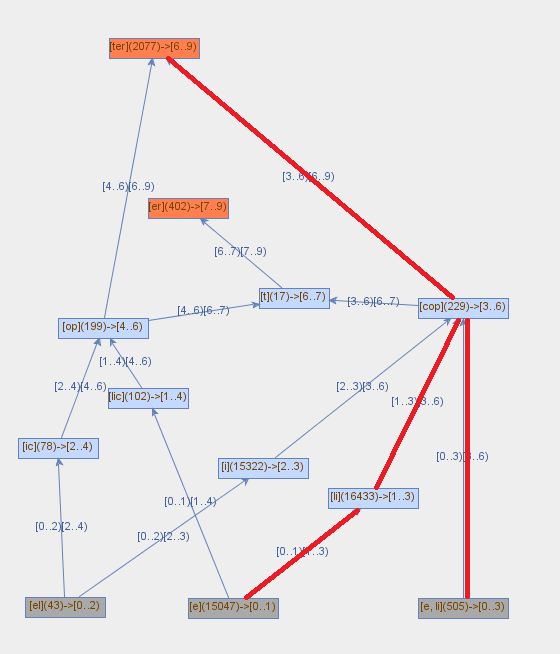
\includegraphics[width=0.7\textwidth]{figures/rosil-counting.png}
    \caption{Aplicarea strategiei numărului de lanțuri închise pentru $G_{elicopter}$}
    \label{fig:rosil-counting}
\end{figure}

\subsection{Strategie bazată pe nivelul de suprapunere}

O altă strategie pornește de la presupunerea că un nivel ridicat de suprapunere la între tiparele unui lanț închis duce la o mai bună predicție a silabisirii unui cuvânt.

\begin{defi}
Având două tipare potrivite în cadrul unui cuvânt la pentru intervalul de îndexi $[i_{p_1}, j_{p_1})$, respectiv $[i_{p_2}, j_{p_2})$ de definește nivelul de potrivire al acestor două tipare ca fiind:
\begin{equation}
\omega(p_1, p_2) = \left\{
\begin{matrix}
0, 					& j_{p_1} \leq i_{p_2}\\ 
max(i_{p_2},j_{p_1)} - min(j_{p_2},i_{p_1}),	& j_{p_1} > i_{p_2} \\
\end{matrix}
\right.
\end{equation}
\end{defi}

\begin{ex}
Pentru tiparul $p_1$ potrivit la întervalul $\left[0, 6\right)$ și tiparul $p_2$ potrivit la întervalul $\left[4, 8\right)$ avem $ \omega(p_1,p_2)=2$
\end{ex}

\begin{defi}
Fie $p_1, p_2, ..., p_n$ un lant de tipare închis $l$. Nivelul de suprapunere pentru întreg lanțul este:
\begin{equation}
\Omega(l) = \sum_{i=1}^{n-1}{ \omega(p_i, p_{i+1})}
\end{equation}
\end{defi}

Pornind de la definiția nivelului de suprapunere de la nivelul unui lanț de tipare închis, se poate realiza o ordonare in funcție de acest nivel a lanțurilor închise din cadrul unui graf de tipare al unui cuvânt, iar ulterior să se propună ca silabisire a acelui cuvânt, silabisirea asociată cu lanțul închis cu nivel maxim de suprapunere. Această strategie este ilustrată în cadrul \ref{fig:rosil-overlapping}.


\begin{figure}[h!]
    \centering
    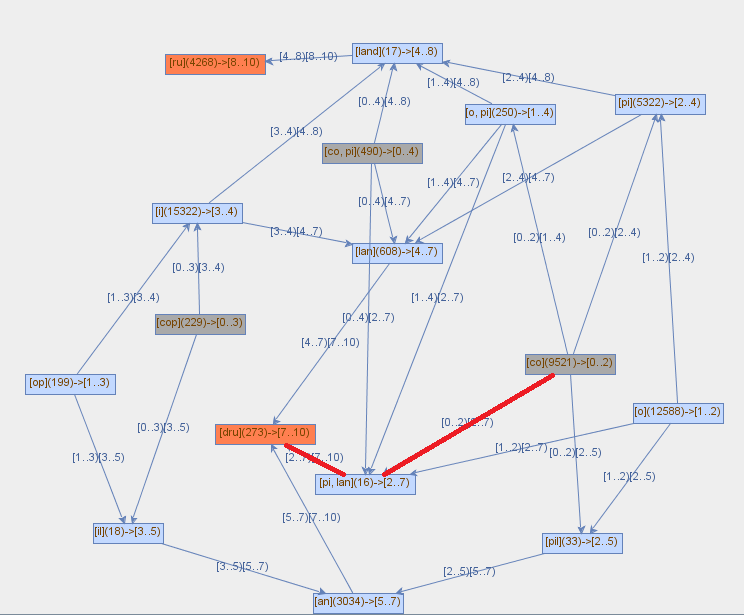
\includegraphics[width=0.9\textwidth]{figures/rosil-overlapping.png}
    \caption{Aplicarea strategiei bazate pe nivelul de suprapunere pentru $G_{copilandru}$}
    \label{fig:rosil-overlapping}
\end{figure}

\subsection{Strategie bazată pe distanța dintre nodurile extreme}

A treia strategie propusă încearcă să exploreze presupunerea că, cu cât sunt mai lungi tiparele dintr-un lant închis, cu atât creste probabilitatea ca acest lanț să aibă asociată o silabisire corectă.

Dar cum s-ar putea identifica aceste lanțuri? Un posibil răspuns la această întrebare vine de la observația că lungimea medie a tiparelor dintr-un lanț inchis este invers proporțioanală cu lungimea lanțului. 

Atfel, acestă stategie selecția acelor lanțuri de lungime minimă. Deasemenea, în cazul în care există mai multe lanțuri de lungime minimă, se va alege acela care prezintă mai mai mare grad de suprapunere. 

\begin{ex}
În cadrul figurii \ref{fig:rosil-shortest} este ilustrată aplicarea acestei strategii. 
\end{ex}

\begin{figure}[h!]
    \centering
    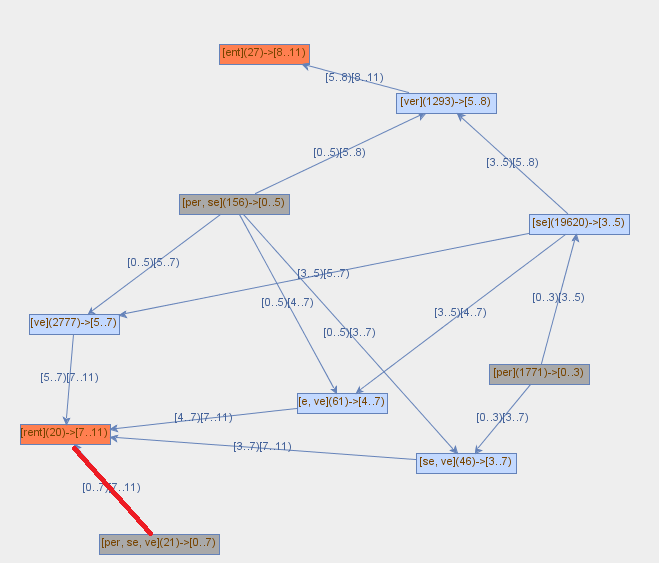
\includegraphics[width=0.9\textwidth]{figures/rosil-shortest.png}
    \caption{Aplicarea strategiei drumului minim pentru $G_{perseverent}$}
    \label{fig:rosil-shortest}
\end{figure}

\section{Metrici de evaluare}

Odată definite strategiile de mai sus, acestea trebuie validate, iar pentru a le valida, se vor defini doua metrici.

\subsection{Evaluare la nivel de cuvânt}


Cea mai simplă variantă este de a considera de a trata despărțirea în silabe ca fiind atomică.

\begin{defi} Fie $w$ un cuvânt, iar $s_p$ o silabisire posibilă a acestui, și $s_e$ silabisirea corectă. Atunci, se definește metrica de evaluare a silabisirii propuse ca fiind:

\begin{equation}
m_w(s_p,s_e) = \left\{
\begin{matrix}
0, 	& $ dacă $ s_p=s_e\\ 
1,	& $ dacă $ s_p\neq s_e \\
\end{matrix}
\right. 
\end{equation}
\end{defi}

\subsection{Evaluare la nivel de punct de despărțire}

În anumite cazuri există mai multe despărțiri în silabe corecte (în funcție de context), este necesară si definirea unei metrici cu o granularitate mai mică.

\begin{defi}
Fie $s$ o despărțire în silabe a unui cuvânt. Mulțimea punctelor de despărțire echivalente despărțirii $s$ este colecția de indexilor acelor litere din cuvânt, care au înaintea lor un punct de despărțire. De exemplu pentru despărțirea $a-ma-tor$, mulțimea punctelor de despărțire este $\{1,3\}$.
\end{defi}


\begin{defi}
Considerând mulțimea indexilor de despărțire $I_{s_p}$ pentru o silabisire $s_p$ a unui cuvânt, iar $I_{s_e}$ mulțimea indexilor despărțirii corecte a aceluiași cuvânt, se definește metrica $m_d$:

\begin{equation}
m_d(s_p,s_e) = 1- \frac{\vert I_{s_e} \setminus I_{s_p} \vert}{2 \cdot \vert I_{s_e} \vert} - \frac{\vert I_{s_p} \setminus I_{s_e} \vert}{2 \cdot \vert I_{s_p} \vert}
\end{equation}
\end{defi}

Interpretarea metricii de mai sus depinde de două componente: numărul de puncte de despărțire prezise corect și numărul de puncte de despărțire prezise gresit.

\begin{ex}
Pentru o mai bună întelegere, fie următoarele exemple:

\begin{equation}
m_d(\{1,3,5\}, \{2,4,6\}) = 1- \frac{3}{2 \cdot 3} - \frac{3}{2 \cdot 3} = 0 
\end{equation}

\begin{equation}
m_d(\{1,3,5\}, \{2,3,6\}) = 1- \frac{2}{2 \cdot 3} - \frac{2}{2 \cdot 3} \simeq 0.33 
\end{equation}

\begin{equation}
m_d(\{1,3,5\}, \{2,3,5\}) = 1- \frac{1}{2 \cdot 3} - \frac{1}{2 \cdot 3} \simeq 0.66 
\end{equation}


\begin{equation}
m_d(\{1,3,5\}, \{1,3,5\}) = 1 - \frac{0}{2 \cdot 3} - \frac{0}{2 \cdot 3} = 1 
\end{equation}


\end{ex} 

\section{Algoritm de silabisire folosind tipare secvențiale frecvente}
În \ref{algo:rosil} este ilustrat algoritmul complet prin care se poate identifica silabisirea unui cuvânt pornind de la o colecție de tipare secvențiale frecvente și o strategie prin care se alege o silabisire din cadrul mulțimii silabisirilor posibile identificate pe baza tiparelor frecvente.
\begin{algorithm}
\SetAlgoLined
\SetKwFunction{ppg}{splitWord}

\ppg($P, w, s$) \\
\KwData{$P$ o colecție de tipare secvențiale frecvente, $w$ cuvântul care se dorește a fi despărțit în silabe, $selectionStrategy$ o strategie de selecție a unei silabisiri din cadrul unei colecții de lanțuri închise de tipare}
\KwResult{$s_w$ o silabisire a cuvântului $w$} 

$M_w = findMatchingPatterns(P,w)$ \\
$G_w = buildMatchedPatternsGraph(M_w)$ \\
$Gp_w = prune(G_w)$ \\
$L_w = findClosedPatternChains(Gp_w)$ \\
\KwRet $pickSolution(L_w, selectionStrategy)$
\vspace{.1cm}

\caption{Predicția despărțirii în silabe ale unui cuvânt $w$}
\label{algo:rosil}
\end{algorithm}

\chapter{Detalii de proiectare si implementare}

În vederea validării ideilor mai sus prezentate, a fost realizată o implementare în limbajul Java care este descrisă în cele ce urmează.

\section{Tehnologii utilizate}

Soluția a fost implementată folosind următoarele tehnologii:

\begin{itemize}
	\item \textit{JDK 8} ~\footnote{https://jdk8.java.net/}
	\item \textit{Gradle} ~\footnote{https://gradle.org/} (pentru compilare si impachetare)
	\item \textit{Git} ~\footnote{https://git-scm.com/} (pentru versionare)
\end{itemize}

La nivel de librarii Java au fost folosite următoarele librarii:

\begin{itemize}
    \item \textit{com.google.guava:guava:18.0} (pentru colecții)
	\item \textit{org.apache.commons:commons-lang3:3.4} (pentru manipulare de siruri de caractere)
    \item \textit{com.google.code.gson:gson:1.7.2} (pentru serializare JSON)
	\item \textit{org.jgrapht:jgrapht-dist:0.9.1} (pentru visualizare de grafuri)
	\item \textit{jp.ac.titech.cs.se:sparesort:0.2.0} (pentru identicarea de tipare secvențiale frecvente)
	\item \textit{org.apache.logging.log4j:log4j-core:2.3} (pentru logare)
    \item \textit{junit:junit:4.12} (pentru unit-teste)
\end{itemize}

Codul sursă al projectului poate fi consultat la urmatoarea adresa: \begin{center}
\textbf{\href{https://github.com/adrianulbona/rosil}{https://github.com/adrianulbona/rosil}}
\end{center}

\section{Organizarea aplicației}

Aplicația implementată în cadrul acestui proiect este organizată în patru pachete, ilustrate în figura \ref{fig:rosil-packages}.

\begin{figure}[h!]
    \centering
    
\includegraphics[width=0.7\textwidth]{figures/rosil-packages.png}
    \caption{Pachetele Java ale prototipului implementat}
    \label{fig:rosil-packages}
\end{figure}

Pachetul \textit{input} este utilizat pentru a citi setul de cuvinte silabisite si pentru al pregatii pentru procesari ulterioare. Pachetul \textit{pattern} are ca principala responsabilitate identificarea tiparelor secvențiale frecvente din cadrul cuvintelor deja sibabisite si incărcate cu ajutorul pachetului \textit{input}. Componenta de predicție este localizată în cadrul pachetului \textit{predict}, iar în cadrul pachetului \textit{eval} au fost implementate o serie de metrici necesare validarii diverselor strategii de predictie.

Pachetul \textit{predict} este deasemenea compus din mai multe sub-pachete care sunt ilustrate în diagrama ~\ref{fig:rosil-predict-packages}. Sub-pachetul \textit{match} are ca responsabilitate identificarea tiparelor (dintr-o colectie de tipare) care potrivesc un anumit cuvânt, sub-pachetul \textit{graph} modeleaza grafuri de tipare potrivite, în cadrul sub-pachetului \textit{chain} conține abstractizari pentru lanțuri de tipare, iar sub-pachetul \textit{strategy} conține implementari pentru strategiile de selecție ale unei silabificari dintr-o colecție de lanțuri de tipare. 

\begin{figure}[h!]
    \centering
    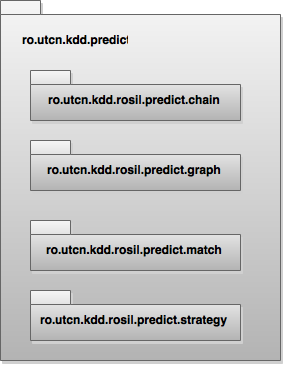
\includegraphics[width=0.3\textwidth]{figures/rosil-predict-packages.png}
    \caption{Pachetele Java ale prototipului implementat}
    \label{fig:rosil-predict-packages}
\end{figure}
\subsection{Structuri de date}

\subsection{Modularizare}
